%!TEX root = ../thesis.tex
Although jamming might seem as a novel approach in the area of HCI, other areas of research have had it on their agenda for some time. 
Especially in the area of mechanical engineering where the jamming mechanism has shown promising results in robotic applications as a substitute for mechanical parts.
In the following we cover the current applications of jamming in both HCI and engineering. 

\subsubsection{Mechanical engineering and robotics}

\citet{brown2010universal, amend2012positive} used the jamming technique to develop a universal robotic gripper \hl{derudover 15,17,18,19 fra referencer i det paper}. 
A gripper is the tool at the end of a robotic arm that interacts with its environment.
This gripper was simply build with an elastic bag as a container for the granular material, which was chosen to be grounded coffee. 
It is able to pick up objects of heterogeneous shapes due to the gripper simply adapting to the surface structure of the objects on impact, see figure~\ref{fig:ch:jamming:jamming-robot-gripper}. 
\todo{this is cool because\dots 1-degree freedom $\rightarrow$ modulated into multi DoF}

\begin{figure}
	\centering
  		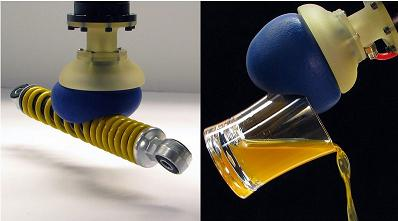
\includegraphics[width=4in]{figures/jamming/jamming-robot-gripper}
	\caption[A universal robotic gripper based on the jamming of granular material by \citet{brown2010universal}.]
   {A universal robotic gripper based on the jamming of granular material.}
   \label{fig:ch:jamming:jamming-robot-gripper}
\end{figure}

Jamming is also seen in experiments with autonomous robots where the mechanism be can used as artificial muscles.

\citet{steltz2009jsel} used the jamming technique to create a platform for shape-changing and mobile robots called JSEL (Jamming Skin Enabled Locomotion).
The soft robot can morph its ``skin'' to create movement of the entire body. 
As opposed to the other applications mentioned this work is based on a division of cells, each of which can be jammed and unjammed to create movement, see figure~\ref{fig:ch:jamming:jsel}. 

\citet{steltz2010jamming} took the JSEL approach further combining the cell-based approach with a linear actuator. 
The assembly combines the contraction and extension capabilities of the linear actuator and modulates this 1-degree of freedom (DoF) actuation into a multi-DoF actuator depending on the number of surrounding jamming cells.
The platform is called JMU (Jamming Modulated Unimorph) and has been tested as component segments of a worm, as an example of a soft robot (see figure~\ref{fig:ch:jamming:jmu}).

These different examples from other fields of research illustrate how creative implementations of the jamming technique and adding other layers of actuation can extend the applicability of jamming.
\todo{purpose $\to$ human unfriendly environments}

\begin{figure}
  \centering
  \begin{minipage}[t]{.45\textwidth}
    \centering
    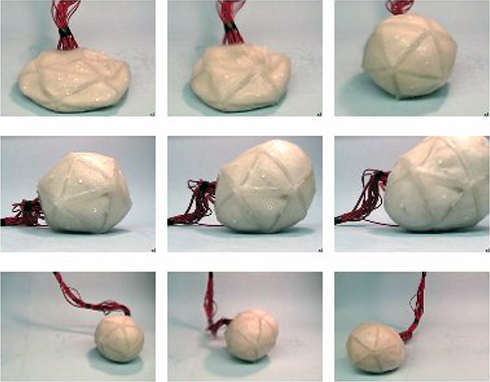
\includegraphics[width=.9\linewidth]{figures/jamming/chembot-robot-blob}
    \caption[Jamming Skin Enabled Locomotion (JSEL) by \citet{steltz2009jsel}.]
    {Jamming Skin Enabled Locomotion (JSEL). Each cell can be jammed individually to create motion.}
    \label{fig:ch:jamming:jsel}
    \hspace{.2\textwidth} 
  \end{minipage}%
  \hspace{0.5cm}
  \begin{minipage}[t]{.45\textwidth}
    \centering
    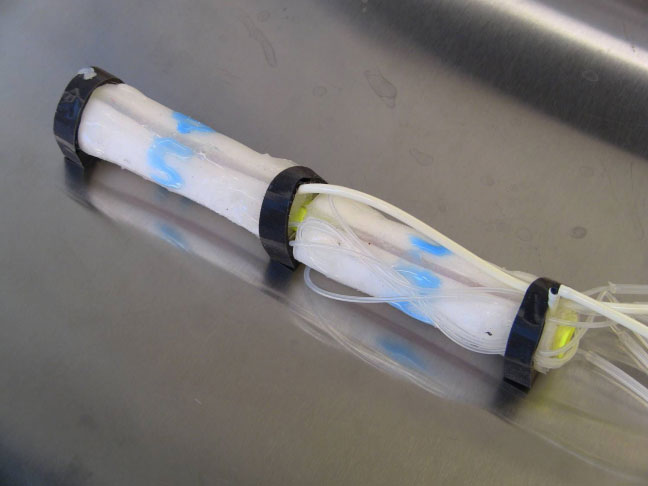
\includegraphics[width=.9\linewidth]{figures/jamming/jmu-worm}
    \caption[Jamming Modulated Unimorph by \citet{steltz2010jamming}.]
    {Jamming Modulated Unimorph.}
    \label{fig:ch:jamming:jmu}
  \end{minipage}
\end{figure}

\subsubsection{Human-computer Interaction}
\label{ch:jamming:related-work:hci}
There are only a few research papers published with emphasis on jamming in Human-computer Interaction (HCI). \todo{\dots}
%Table~\ref{ch:jamming:tab:applications_overview} on page \pageref{ch:jamming:tab:applications_overview} shows an overview of the applications mentioned in this section.

\paragraph{The HoverMesh}
\label{ch:jamming:related-work:hci:hovermesh}
\citet{mazzone2004hovermesh} did some early work on creating a deformable structure with the jamming technique. 
The HoverMesh prototype is a cell-based jamming system consisting of 3x3 grid, see figure~\ref{fig:ch:jamming:hovermesh}.
The grid is mounted on top of a cubicle which can be inflated and deflated and together with the grid it creates deformations of the surface structure.
The HoverMesh prototype is not fully implemented according to the ideas presented.
It consists only of the grid structure on top of the cubicle and does not exhibit input capabilities through vision-based techniques and haptic feedback output as intended. 
\todo{A bit of a primitive construction. But }

\paragraph{ClaytricSurface}
\label{ch:jamming:related-work:hci:claytric}
\citet{matoba2012claytricsurface} created a flexible tabletop surface, ClaytricSurface, which serves as a sculptable display medium, see figure~\ref{fig:ch:jamming:claytric-surface}. 
The surface can be directly manipulated by hand and the stiffness can be controlled in real time by a GUI slider.
The exemplified application in this short paper is a painting application projected onto the surface from above and a user can use direct touch on the surface to draw. 
The input is detected by a depth camera from above the tabletop.
\todo{critical points: depth camera and project. and application - 1-page-paper though, it exists in a longer version in Japanese}
\todo{the videos give a more artistic impression of the applicability.}

\begin{figure}
  \centering
  \begin{minipage}[t]{.4\textwidth}
    \centering
    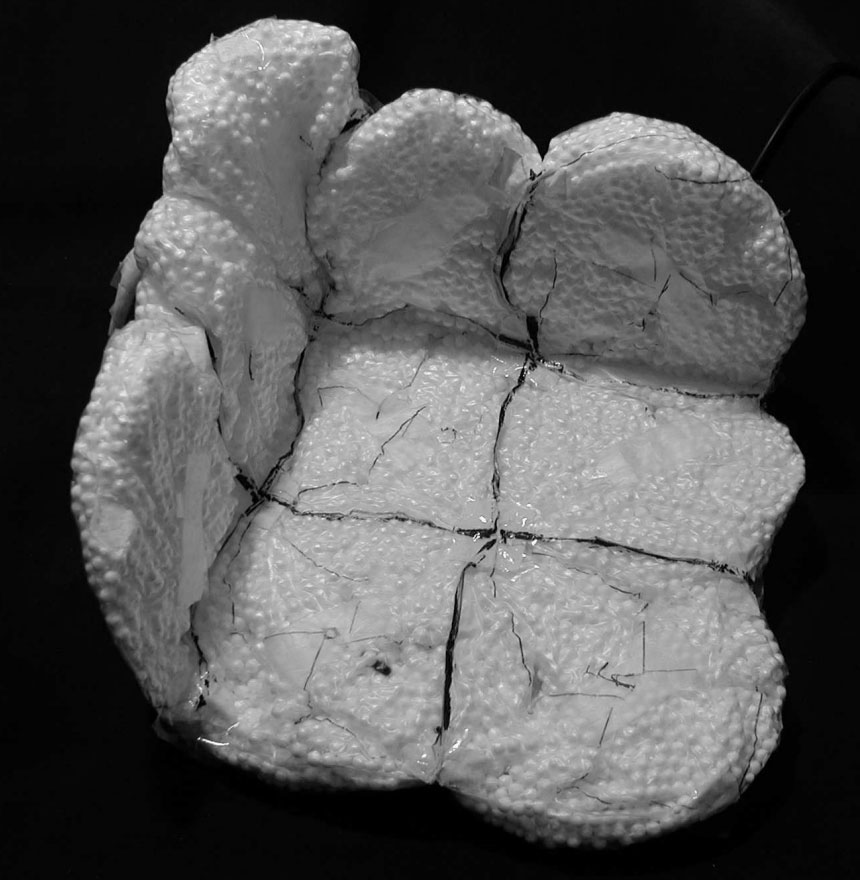
\includegraphics[width=.9\linewidth]{figures/jamming/hovermesh}
    \caption[The HoverMesh by \citet{mazzone2004hovermesh}.]
    {The HoverMesh.}
    \label{fig:ch:jamming:hovermesh}
  \end{minipage}%
  \hspace{0.5cm}
  \begin{minipage}[t]{.4\textwidth}
    \centering
    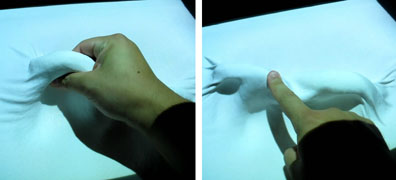
\includegraphics[width=.9\linewidth]{figures/jamming/claytric-surface}
    \caption[Claytric Surface by \citet{matoba2012claytricsurface}.]
    {Claytric Surface.}
    \label{fig:ch:jamming:claytric-surface}
  \end{minipage}
\end{figure}

\paragraph{Jamming User Interfaces}
\label{ch:jamming:related-work:hci:jui} 
\citet{follmer2012jamming} has probably made the biggest contribution yet to the use of jamming in HCI. 
The authors coin the approach \textit{Jamming User Interfaces} and position it in the area of malleable and organic user interfaces. 
They make several contributions to the field by exploring jamming interfaces for haptic feedback, for malleable tabletops and for mobile devices, see figure~\ref{fig:ch:jamming:jui-collection}. 
They also investigate how sensing techniques like capacitive and optical sensing, can broaden the applicability of jamming in HCI. 

\citet{follmer2012jamming} also present a hydraulic jamming system that is fast and silent and which allow for transparent jamming volumes. 
This requires transparent particles and a transparent fluid that matches the refractive index of the particles so that light refraction is reduced. 
\todo{maybe an image here}

\todo{critical points: very much proof on concept, misses real world implementations.}

In the following we will give a brief overview of the four prototypes implemented and described by \citet{follmer2012jamming}.

\subparagraph{Tunable Clay} is a malleable tabletop for direct 3D modelling, see figure~\ref{fig:ch:jamming:jui-clay}
It resembles ClaytricSurface \citep{matoba2012claytricsurface} mentioned earlier with is clay-like surface that can easily be deformed.
Tunable Clay uses the hydraulic jamming system mentioned above with index-matched particles and fluid.
This allows for a more sophisticated depth sensing approach than the one used with ClaytricSurface.
Optical shape sensing and graphic projection is integrated underneath the jamming volume.
The shape, captured in real-time, is shown as a virtual 3D model on both an external display and on the jamming volume itself projected from underneath the surface.

\subparagraph{Transparent Haptic Lens} is small tangible puck to be used as a haptic information channel on a tabletop display, see figure~\ref{fig:ch:jamming:jui-lens}.
It has a transparent lens in the center which is a transparent hydraulic jamming volume which can change its stiffness according to the texture beneath it.
A user presses \todo{a/his/hers} finger into the lens to get a haptic sensation about the underlying texture of the image directly underneath. 

\subparagraph{Behind-the-Tablet Jamming} is a tablet computer which has a pneumatic jamming volume mounted on the backside, see figure~\ref{fig:ch:jamming:jui-tablet}.
The system senses malleable input with capacitive shape sensing.
The scenarios envisioned are for navigating content (e.g. scrolling and zooming) on the tablet display through malleable interaction on the backside. 
The system can communicate that some limit is reached with haptic feedback, 
e.g. by stiffening the jamming volume.

\subparagraph{ShapePhone} is a generic mobile device that can be shaped and locked into different forms, see figure~\ref{fig:ch:jamming:jui-phone}.
The device has no technology inside, except for the jamming system, and it merely serves as demonstration of how its affordances change when it is sculpted into forms resembling e.g. a phone, remote control or a watch.
Ideas are presented for integrating various sensing techniques such as capacitive shape sensing and touch sensing to derive contextual information.

\begin{figure}
        \centering
        \begin{subfigure}[b]{0.45\textwidth}
                \centering
                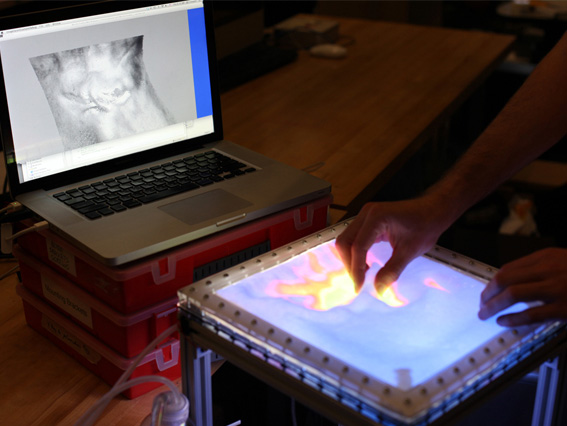
\includegraphics[width=\textwidth]{figures/jamming/jui_tunable-clay}
                \caption{Tuneable Clay}
                \label{fig:ch:jamming:jui-clay}
        \end{subfigure}
        \begin{subfigure}[b]{0.45\textwidth}
                \centering
                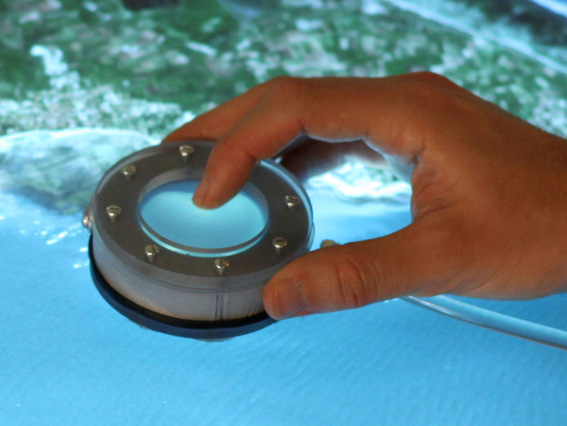
\includegraphics[width=\textwidth]{figures/jamming/jui_haptic-lens}
                \caption{Transparent Haptic Lens}
                \label{fig:ch:jamming:jui-lens}
        \end{subfigure}

        \begin{subfigure}[b]{0.45\textwidth}
                \centering
                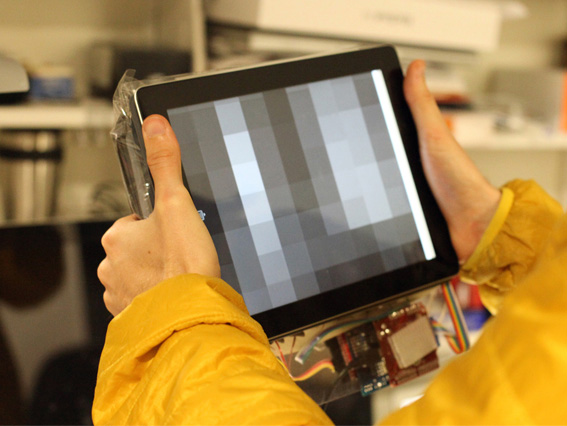
\includegraphics[width=\textwidth]{figures/jamming/jui_behind-the-tablet}
                \caption{Behind-the-Tablet Jamming}
                \label{fig:ch:jamming:jui-tablet}
        \end{subfigure}
        \begin{subfigure}[b]{0.45\textwidth}
                \centering
                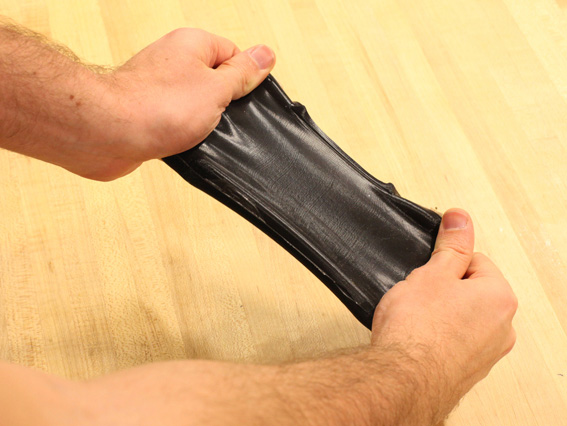
\includegraphics[width=\textwidth]{figures/jamming/jui_shapephone}
                \caption{ShapePhone}
                \label{fig:ch:jamming:jui-phone}
        \end{subfigure}
        \caption{Jamming User Interfaces by \citet{follmer2012jamming}.}
        \label{fig:ch:jamming:jui-collection}
\end{figure}

\subsection{Summary}

In the previous sections we have given an introduction to the mechanics of jamming and an overview of different research applications of jamming.
These applications show two primary approaches to jamming.
The first one is the basic approach where a single volume containing particles can be jammed by applying a vacuum inside, see figure~\ref{fig:ch:jamming:approaches:basic}.
Applications of the basic approach are for example, \emph{Claytric Surface} and \emph{ShapePhone}.
The other is the more complicated cell-based approach where each cell is an independent jammable volume working in the same manner as the basic approach.
As the cells exist on the perimeter of the volume some other compound must constitute the body of the volume and stabilise the form.
In \emph{The HoverMesh} this was air inside a cubicle and in \emph{JSEL} it was fluid, see figure~\ref{fig:ch:jamming:approaches:cell}.

\begin{figure}
  \centering
  \begin{minipage}[t]{.45\textwidth}
    \centering
    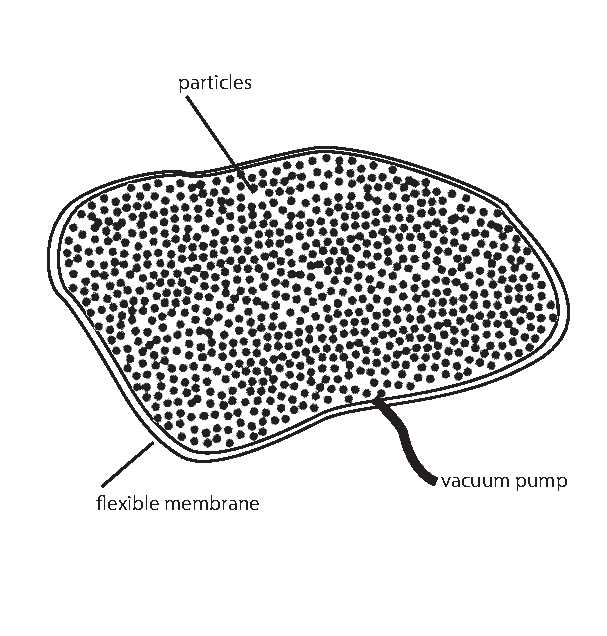
\includegraphics[width=.9\linewidth]{figures/jamming/basic_jamming}
    \caption[The basic jamming approach.]
    {Illustrates the basic approach with a single jammable volume.}
    \label{fig:ch:jamming:approaches:basic}
  \end{minipage}%
  \hspace{0.5cm}
  \begin{minipage}[t]{.45\textwidth}
    \centering
    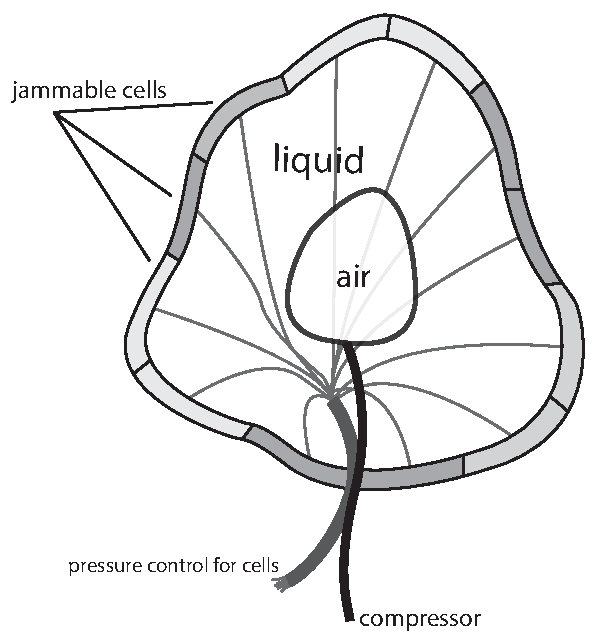
\includegraphics[width=.9\linewidth]{figures/jamming/cell_jamming}
    \caption[The cell-based jamming approach.]
    {Illustrates the cell-based approach where each cell functions as an independent jammable volume.}
    \label{fig:ch:jamming:approaches:cell}
  \end{minipage}
\end{figure}

Table \ref{ch:jamming:table:applications_overview} summarises and categorises the mentioned applications according to their characteristics.
In the next we will move on to our own concepts that support the notion of ad hoc interfaces.

\begin{landscape}
  \thispagestyle{empty}
  \centering 
  \captionof{table}{An overview of jamming in HCI}
  \label{ch:jamming:table:applications_overview} 
  \begin{tabularx}{\linewidth}{|l|c|c|c|c|c|X|}
    \hline
    Project                 & Input                         & Output                        & Type      & Particles   & Approach  & Summary \\ \hline
    \hline
    Robotic gripper         & \cellcolor{FalseColor}\xmark  & \cellcolor{TrueColor}\cmark   & pneumatic & coffee      & basic     & A universal robotic gripper \\ \hline
    Jamming Skin Enabled Locomotion & \cellcolor{FalseColor}\xmark  & \cellcolor{TrueColor}\cmark   & pneumatic & glass beads     & cell-based& A soft moving robot \\ \hline
    Jamming Modulated Unimorph & \cellcolor{FalseColor}\xmark  & \cellcolor{TrueColor}\cmark   & pneumatic & glass beads          & cell-based& A worm-like robot \\ \hline
    \hline
    The HoverMesh           & \cellcolor{FalseColor}\xmark  & \cellcolor{TrueColor}\cmark   & pneumatic & polystyrene & cell-based& A cell-based deformable surface structure . \\ \hline    
    ClaytricSurface         & \cellcolor{TrueColor}\cmark   & \cellcolor{FalseColor}\xmark  & pneumatic & polystyrene & basic     & A flexible tabletop surface which serves as a sculptable display medium. \\ \hline
    Tunable Clay            & \cellcolor{TrueColor}\cmark   & \cellcolor{FalseColor}\xmark  & hydraulic & glass beads & basic     & A malleable tabletop for direct 3D modelling. \\ \hline
    Transparent Haptic Lens & \cellcolor{FalseColor}\xmark  & \cellcolor{TrueColor}\cmark   & hydraulic & glass beads & basic     & A small tangible puck to be used as a haptic information channel on a tabletop display. \\ \hline
    Behind-the-Tablet       & \cellcolor{TrueColor}\cmark   & \cellcolor{TrueColor}\cmark   & pneumatic & ?           & basic     & A tablet with a interactive jamming volume on the back. \\ \hline
    ShapePhone              & \cellcolor{TrueColor}\cmark   & \cellcolor{FalseColor}\xmark  & pneumatic & coffee      & basic     & a generic mobile device that can be shaped and locked into different forms. \\
    \hline
  \end{tabularx}

  \begin{flushleft}
  This table is an overview of the prototypes presented in the papers covered in this section. It should be mentioned that in categorising \textit{input} and \textit{output} features we are only considering whether input or output is enabled using the jamming technique. For example, \textit{Tunable Clay} does have output in the form a image projection but it does not utilise the jamming technique.
  \todo{information is of course retrieved from the papers but some parts are not available. Check other sources: web pages, videos, email author??}
  \end{flushleft}

\end{landscape}
